\documentclass{article}

% The geometry package allows for easy page formatting.
\usepackage{geometry}
\geometry{letterpaper}

% Load up special logo commands.
\usepackage{doc}

% Package for formatting URLs.
\usepackage{url}

% Packages and definitions for graphics files.
\usepackage{graphicx}
\usepackage{epstopdf}
\DeclareGraphicsRule{.tif}{png}{.png}{`convert #1 `dirname #1`/`basename #1 .tif`.png}
%
% Set the title, author, and date.
%
\title{The Smartime Smart Watch}
\author{Joaquin Loustau}
\date{November 27, 2014}

%
% The document proper.
%
\begin{document}

% Add the title section.
\maketitle

% Add an abstract.
\abstract{A User Interface (UI) in computing refers to how a computer program or system represents itself to its user, usually via graphics, text and sound. The key feature of wearable UI is that it should keep your hands free and not hinder your daily activities. In other words, it should serve as a secondary activity for you, as and when you wish to access it. This essay describes a 'dream' user interface for a smart watch, the Smartime.
}

% Add various lists on new pages.
\pagebreak
\tableofcontents

% Start the paper on a new page.
\pagebreak

%
% Body text.
%
\section{Description}
The wristwatch has been an ever-present wearable technology since its inception in the late 1800s, and has undergone continuous technical refinements since that time. Researchers have long viewed the immediacy and ubiquity of the wristwatch as a vehicle for computation, pushing its capabilities to ever-greater heights. In 2000, IBM demonstrated the first watch running a full operating system.\cite{amft2009backpacks}  

One of the main reasons wristwatches emerge as attractive wearable devices is the fact that a large fraction of the population is already accustomed to wearing them, thus favoring the learning curve for novice users. Furthermore, people generally keep watches on their wrists, so watches are less prone to be misplaced compared to phones and tablets. For example, a hip holster or pocket are not convenient places to keep a cellular phone while sitting in a car, and so people tend to keep them in the car seat and forget them when they leave the car in the parking lot. 

Another significant advantage of a wrist watch is that it is much more accessible than many of the other devices one may carry. It is often said that one of the reasons for the initial success of the Palm was its moving to an instant-on paradigm, i.e. eliminating the long boot up time associated with laptops. Wrist watches move users to the next step: an instantly-viewable paradigm.

The primary challenge faced by wearable devices in general and smart watches in particular is the lack of an adequate User Interface (UI). The smart phone suffered a similar problem in its origins. An adequate smart phone user interface was missing for a long time until the development of the iPhone --its adequate interface being the reason it was superior to all other approaches at that time. The same challenge is ahead for this new class of device: the smart watch. 

Unlike smart phones, which can be scaled to a variety of sizes, smart watches must be small and unobtrusive in order to remain socially acceptable and practical for the user. The reduced size of the screen poses challenges to the possibilities and usability of multi-touch technology. One approach, followed most notably by Google, is voice recognition.  However, it does not yet appear to be socially acceptable to talk to a watch. In addition, in environments with high noise pollution, its accuracy falls dramatically. This is particularly true of devices such as the Samsung Gear, as its microphones are tuned to support surrounding noise for its video recording feature.

Another approach some devices such as the Moto 360 and Apple Watch have employed is to make use of a gyroscope to recognize when users turn their wrist to look at the device so as to lighten up the watch face. This feature provides the foundations for a technology which emulates the most intuitive movements we do with our hands and arms - touching and pointing to something. This technology is further explored in the Design section.

The User Interface design below aims to enhance the most important capabilities of existing smart watches while eliminating aspects and features that proved to be impediments to usability purposes. The interface described also includes a couple of features that are not yet part of any smart watch, but due to undergoing research, will be feasible in the near future. 


\section{Design}
The watch designed, named Smartime, stays true to the timeless form of the classic wristwatch. A round design maximizes the display area and, unlike the Moto 360, effectively makes use of 100\% of the screen.

\begin{figure}[h]
\centering
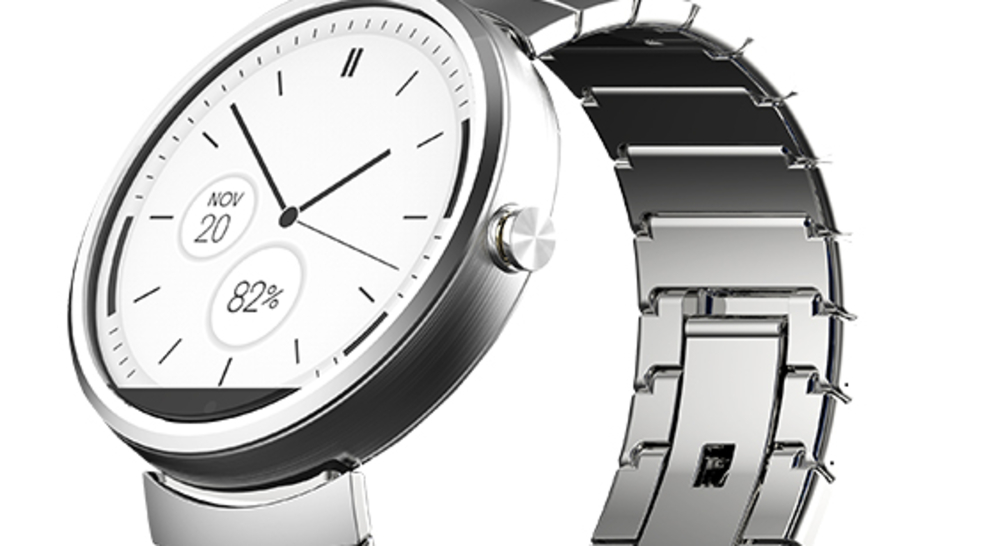
\includegraphics[width=3 in]{moto360_screen.jpg}
\caption{The screen of the Moto 360 is not used completely. The bottom of the screen remains black and therefore does not fully exploit its round screen. }
\end{figure}

In order to expand accessibility, two almost identical versions of Smartime accommodate both users that use their watch on their left arm (usually right-handed) and those who wear it on their right hand (frequently left-handed). The only difference between the two models is that the digital crown and fingerprint reader tip are interchanged -the digital crown is on the same side of the watch as the hand that is free.

Since wristwatches were invented in the 19th century, people have been glancing at them to check the time. With Smartime, this simple, reflexive act allows users to learn so much more. Smartime offers users the possibility to access scannable summaries of the information they seek out most frequently. These will very similar to the cards in the Context Stream: short snippets of relevant information, with an optional photo backdrop. Users will be able to swipe up to see expanded information.

 To switch between cards, users simply swipe to the sides from the current screen. Users can tap on one of these cards to go directly to its corresponding app for more details. This makes navigation fluid and responsive.

Smartime has a built-in ambient light sensor such as the one found in the Moto 360. When the sensor is enabled, the device automatically adjusts the screen back-lighting according to the environment.This feature saves the user having to access the settings to increase or decrease the screen brightness whenever the lighting conditions change. It also optimizes battery life by automatically reducing the power requirement based on real time conditions.
 
Smartime organizes users' information by predicting what they need, when they need to see it and displaying it before they even ask -always avoiding an overflow of notifications.  Users receive real-time notifications -in the form of a gentle tap- for incoming mail, messages, and calls. From the watch, they are able to decide whether to dismiss them or answer them (either on a phone or on the watch itself).

If the user decides to answer a text message on the phone, he will have three options. First, he will be able to choose from a list of 4 or 5 text messages produced by the watch's software based on the incoming message. For example, if the incoming message includes the words ``What time...,'' the sample messages will most likely be an array of times of the day. In other words, Smartime analyzes the incoming message, attempts to understand its meaning and produce possible answers. All this computation occurs on the device itself and, unless specifically requested, is stored only on the device.  Second, if none of the custom messages offered by Smartime satisfies the user, he is able to select the option to answer by voice command, by tapping on the microphone that will be displayed on the screen. Lastly, the user is able to choose from a diverse group of emoji available.
 
In terms of user interaction, Smartime offers five (5) different ways for the user to interact with the device: 

\begin{enumerate}
\item \textbf{Motion Recognition}\\
A 3-D gesture-recognition chip called Chirp , which is currently being developed at the University of California at Berkeley and the University of California at Davis, will be included inside Smartime. \cite{metz2013} This technology will enable the Smartime watch to recognize complex and precise hand motions and produce content accordingly. The chip uses sonar via an array of ultrasound transducers --small acoustic resonators-- that send ultrasonic pulses outward in a hemisphere, echoing off any objects in their path. Those echoes come back to the transducers, and the elapsed time is measured by a connected electronic chip. When using a two-dimensional array of transducers, the time measurements can be used to detect a range of hand gestures in three dimensions within a distance of about a meter.\\ 

For a smart watch on one's wrist, only short range seems to be necessary. It should be easy to count fingers and determine tilt angle of the other hand placed above it. At near 0 degrees tilt, echo pulses will be closer. At near 90 degrees the returning echo pulses  would indicate 2 fingers tips separated by the time sound travels over an inch. Holding out 2 fingers and turning the tilt from 0 to 90 degree indicate "turn up volume", and the reverse tilt to "turn down volume".\\ 

Another specific example of motion recognition includes making and declining phone calls. When the user receives a call, he is able to decline the call by just shaking the Smartime watch. The Smartime watch will also offer Hands on Talk, the technology for bouncing sound waves off the user's palm when making a call with the watch.
As simple as it may sound, having the user raise his hand to his ear to answer a phone call appears to be more socially acceptable activity as it resembles having a wireless ear bud.

\item \textbf{Digital Crown}\\
This unique input mechanism introduced by the Apple Watch \cite{apple2014} offers phenomenal ``out of the box'' possibilities. On mechanical watches, the crown has historically been used to set the time and date and to wind the mainspring. The Digital Crown allows users to zoom and scroll nimbly and precisely, without obstructing their view. Users can also push it like a button to return to the watch face, making it an integral part of the Smartime watch experience. 

\begin{figure}[h]
\centering
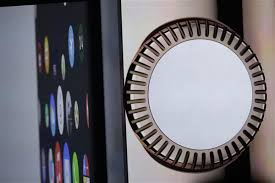
\includegraphics[width=3 in]{digital_crown.jpg}
\caption {Digital Crown on the Apple Watch.}
\end{figure}

\item \textbf{Touch Screen}\\
In addition to recognizing touch, the Smartime watch senses force, adding a new dimension to the user interface. The Force Touch technology, currently used by the Apple Watch, uses extremely small electrodes around the display to distinguish between a light tap and a deep press. This interaction triggers instant access to a range of contextually specific controls -such as an action menu in Messages, or a mode that allows the user to select different watch faces -- whenever the user wants. A short press will be the default command to access advanced settings within the current application.\\

Users can swipe downwards on the screen to cancel a selection or back one screen -when one screen away from the watch face pressing the digital crown and swiping down will have the same effect- and sideways to switch between applications.  


\begin{figure}[h]
\centering
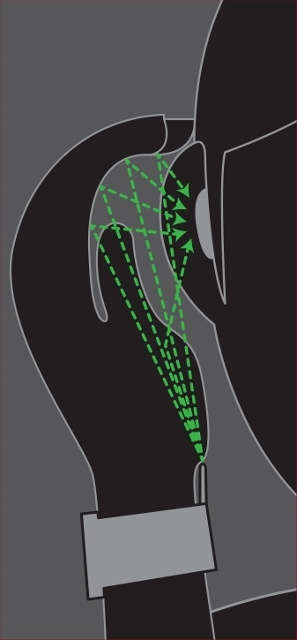
\includegraphics[height=2.5 in]{hotwatch_palm.jpg}
\caption{On Talk technology: sound waves bounce off the user's palm when making or answering a call with the watch.}
\end{figure}

\item \textbf{Voice Recognition }\\
The Smartime watch's voice recognition will provide an accurate and reliable recognition that will allow the user to perform every single action the phone permits -except for authorizing payments- through voice commands. This attempts to provide full functionality to visually impaired users.\\ 

Since the Smartime will not include a video recording feature, the microphone will be configured so as to isolate as much environment noise as possible. Furthermore, in addition to supporting multiple languages, the Smartime watch will support varied accents, a feature no other smart device currently includes.\\ 

By matching the desired language and place of birth of the user, the Smartime watch will adjust its voice recognition to account for an accent original of the user's place of birth. This will make the Smartime watch a device extremely popular overseas and in places with a population of diverse origins.

\item \textbf{Fingerprint Scanner}\\
One of the sides of the Smartime watch has a built-in fingerprint reader tip, similar to those often found on Lenovo Laptops. This feature serves a single but crucial purpose: it allows users to verify their identity when making payments using the watch.  By placing it on the side of the device, the Smartime watch will still keep a stylish minimalist design -indistinguishable from an ordinary device to the common eye.\\

A more thorough explanation of this functionality is provided under the section Usage Scenarios. 

\begin{figure}[h]
\centering
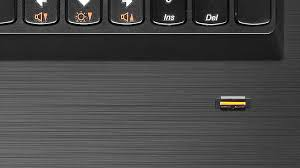
\includegraphics[width=3 in]{lenovo_reader.jpg}
\caption {A fingerprint reader tip like the one found on Lenovo laptops will be included on the side of the watch.}
\end{figure}
\end{enumerate}

In addition to the aforementioned features, the Smartime watch will include another feature that no smart watch in the market currently offers: uninterrupted watch functionality. A significant flaw of present-day smart watches is that when they run out of battery, users do not simply lose just the smart function. The display shuts down, and users lose the ability to even tell time. At this point, devices such as the Moto 360 become nothing more than an expensive bracelet. 

The Smartime watch presents an innovative solution to this problem. Once the battery dies, the watch behaves like an automatic digital watch -the natural movement of the user's arm provides enough energy to keep the watch face and display time accurately. Seiko, Citizen and more recently Ventura have manufactured several generations of automatic digital watches, and extending this technology to a smart watch appears as feasible.

Finally, in terms of battery charging, the Smartime watch will utilize wireless inductive charging technology. Wireless charging functionality, by eliminating the need for a USB port, supports the Smartime design concepts of aesthetic simplicity and maximum usability and convenience. It reduces clutter and promotes a sleek design and also supports the ability to offer a waterproof smart watch.

\section{Usage Scenarios}
\subsection{Office Use}
In office environments, administrators interact both with each other and with various analog and digital devices, making them an interesting space to utilize smart watches.  The Smartime watch's interface offers the possibility of enhancing this kind of environments. \cite{bernaerts2014office}

As smart watches are normally worn on the wrist, there is a significant potential for them to digitally augment gestures performed in day-to-day contexts. The Smartime watch's interface will include an application to assist office employees in easily locking and unlocking doors, in acquiring information and notifying others when they want to enter their office. This application will make use of the motion sensing capability aforementioned. 

The Office application of the Smartime watch implements two types of physical gestures to support the most important functionalities. First, the application provides the opportunity to perform a virtual knock with the same gesture as a real knock.  Alternatively, the interface supports opening/closing doors using the gesture of turning your wrist either clockwise or anti-clockwise, just like turning a key to open or close a door. 

Knowledge workers tend to drop by each other's offices regularly, for example, to ask for assistance or quickly discuss something. Even with the door open, knocking on the door is a common gesture to politely indicate your presence and check whether you are not interrupting the person. Using the smart watch, one could digitally augment these gestures, which can provide a number of benefits. 

For example, when a person is not in his office, knock gestures will still be recognized and transferred to that person's smart watch. This allows office workers to keep a record of who came by and who they might have missed. Additionally, it is often inconvenient to interrupt a phone or Skype conversation to tell the person knocking on the door that it is not a good time. Nevertheless, depending on who is knocking on the door, it might be important enough to interrupt the phone call. Using the smart watch's interface, the person in the call gets a notification about the virtual knock, and can choose to grant or deny their colleague access, without having to interrupt the call. 

Keys (or key cards) are commonly used to open doors in office buildings. However, they present several disadvantages: generic keys could still provide access to restricted rooms; they might be lost or forgotten (e.g. employees could lock themselves out); employees might forget to lock their door, which could lead to theft of personal belongings or sensitive information. The Smartime watch matches the identity of its users to the door they have the rights to open -thus providing more fine-grained access control. Using the user's identity, employees can be granted access only to doors they are allowed to open. Employees do not have to remember to bring their keys with them, assuming they always have their smartwatch on their wrist. To prevent theft, doors could be automatically locked after a specific period of time and door entry and exit could be logged. 

When carrying out gestures, it is difficult to see what is happening on the screen. To address this problem, the Smartime watch adds audio feedback and plays a sound every time a gesture has been detected. Users should be able to immediately distinguish the performed gesture based on the sound they hear. For example, when a virtual knock gesture is performed, the device plays a real knocking sound. For the opening/closing gesture the smart watch uses a rattling keys sound.

Audio feedback will also be generated when someone needs to be notified, like receiving a virtual knock on his device. This is helpful because users might not be looking at their watch at all times. Vibrations are only used sparingly, as they can be distracting to the user. The Office application only uses notifications when someone is knocking on the user's door, when they need to attend a meeting, in case of an error, or when the user tries to perform an action without the valid credentials (e.g. opening the boss' office door). 

\subsection{NFC}
Near field communication, abbreviated NFC, is a form of contact-less communication between devices such as smart phones or tablets. Contact-less communication allows a user to wave the smart phone over a NFC compatible device to send information without needing to touch the devices together or go through multiple steps setting up a connection.

With NFC, a new type of user interface emerges. It is not on the screen anymore, but deeply embedded in the real word. For smart phones, such technology has achieved only limited success because it is convenient to control these devices with the touchscreen. But for devices like a smart watch there will not be a screen of adequate size. Making contact with a NFC tag, which initiates a context-dependent action is the simplest thing to do, especially because the smart watch is placed on the users' wrist, and pointing to or touching something is one of the most intuitive gestures to most individuals. With NFC and smart watches, this gesture has the potential to connect the real and the virtual world in a new and innovative way. Its NFC capability will allow users to share files, such as photos, videos, contacts, etc. by just having their watches in proximity. 

However, the potential uses of NFC go well beyond this. The NFC chip will let users purchase items by just reaching the watch close to a receiver at a cash register. In order to ensure the security of these transactions, each payment will require the user to swipe their finger through the fingerprint sensor, found on the side of the watch. This mechanism emulates the behavior of Apple Play on the iPhone 6 and iPhone 6 Plus. 

Users will also be able to use their rewards cards at different locations, or check in for their flights without the need to extract their phones. The possibilities are endless.




\subsection{Home Automation}
Most smart watches on the market today connect to other devices via low-energy Bluetooth, but not Wi-Fi. That is, in most of the cases, a design decision because battery life would suffer tremendously if wearable devices were constantly searching for a Wi-Fi connection. This has been the main reason halting the development of home automation controlled from a smart watch. However, last June, Broadcom quietly unveiled a new system-on-a-chip that could prove to be a game-changer for the next crop of smart watches due out this year and eventually, for glasses, bio metric sensors and other high-end wearable devices.\cite{murry2014}

The BCM43430 chip family developed by Broadcom has all the features one would expect from a top-notch combo chip, including 2.4 GHz Wi-Fi, Bluetooth 4.1/Bluetooth Smart, FM radio receiver, and a flexible, low-power design. It supports the latest wireless charging standard by the Alliance for Wireless Power, called Rezence, for on-the-go charging. It also has a feature that enables Wi-Fi to exist on a low-power wearable platform.

The secret lies in the chips' ability to orchestrate a behind-the-scenes changeover from Bluetooth to Wi-Fi and back again. ``We believe that the best way to improve the user experience for wearable devices is to leverage both Wi-Fi and Bluetooth,'' Sumit Kharbanda, senior product manager in the Broadband \& Connectivity Group at Broadcom expresses. ``So we have engineered a way to maintain the connection between the two devices. When the user goes out of Bluetooth range, the chip would recognize that and be able to switch over to Wi-Fi before it loses connection,'' he further explains. 

This piece of technology will allow users to fully control all smart devices on their home from the convenience of an application or voice commands on their Smartime watch. Imagine someone driving home from work and without having to move his focus from the road being able to turn on the living room TV, kitchen lights and preheat the oven. With the Smartime watch, this is not only possible; it is extremely easy to do.


\section{Rationale}
Smartwatches promise to bring enhanced convenience to common communication, creation and information retrieval tasks. Due to their prominent placement on the wrist, they must be small and otherwise unobtrusive, which presumably would limit the sophistication of interactions the user can perform. This problem is particularly acute if the smart watch relies on a touchscreen for input, as the display is small and our fingers are relatively large. 

The Smartime watch implements the following Principles of Good Wearable Design in order to overcome the a priori limitations of smart watches.

\begin{enumerate}
\item \textbf{Glances, not stares:} No smart watch should ever command the attention, especially the eyesight, of a user for more than a few seconds at a time. Spending longer erodes any advantage over a smart phone.
\item \textbf{Interact once, display many times:} Smart watches should primarily provide displays of information and prompts for action rather than providing rich interactive elements, meaning they will show lots of information that is passively consumed.
\item  \textbf{Consider User Context:}  Users will not want to be constantly looking at their watches for possible notifications, so the watch will be more effective if it fades into the background and has the right information appear automatically based solely on the context. 
\end{enumerate}

One of the main obstacles smart watches encounter in their path to becoming widely popular devices is the novel behavior they require from users. While certain authors claim that stylish and fashionable devices will ``fix'' smart watches\cite{darmour2012}, this narrative falls apart in the face of decades of study about how new technologies are adopted. As documented by Everett Rodgers in The Diffusion of Innovations, no fundamentally new product type succeeds solely based on the fact that it is attractive; it succeeds because it performs something genuinely useful at a price point low enough that people do not consider it a luxury. 

With fashion off the table, what is standing between today and the smart watches-everywhere future? One thing: a great, unique interface that showcases how much better this new type of wearable device can perform both new and existing functions. Designing an interface for a smart watch requires breaking down functions from devices such as smart phones into small functionalities that allow developers to create simple commands and interactions for users. It requires developing a design approach by looking closely at how to provide the best, most seamless experience for users.

In order to accomplish this goal, the following patterns were identified as requirements for screen navigation, and successfully included to the Smartime watch:

\begin{enumerate}
\item a quick return to the watch face from any application, 
\item a time-out to the watch face from any function,
\item one touch deactivation of alarms, 
\item direct access to the main list of applications, 
\item user programmable touch screen areas that could be used to access the user's most important applications
\item the ability to easy return to the previous screen (People are familiar with the browser model and the concepts of following hyperlinks and going back in the browser history stack. Therefore extending the concept of a browser back button to every watch face screen is desirable)
\end{enumerate}

In conclusion, one aimed to design an interface that enables a clear, logical and seamless usage of the smart watch. In order to design the Smartime watch's interface, Human Computer Interaction (HCI) concepts from familiar computing environments such as web browsers were combined with user-centered design guidelines.


\section{Usability Metrics Forecast}
The Smartime watch was minutely conceived using the results obtained from the usability study of Moto 360 and Pebble carried out for the second assignment of the course. \cite{loustau2014} 

If one of the test subjects who participated in the original study was to perform the tasks using the Smartime watch, he would undoubtedly make fewer mistakes (if any) and would feel an extremely high satisfaction with the interface. The learnability of the Smartime exceeds that of any other smart watch mainly due to the consistency of its interface and the possibility to use several different mechanisms to provide input simultaneously. \cite{akers2014}|

A significant number of test subjects who participated in the usability test mentioned that they were unsure about when they needed to use voice commands and when to tap the screen. Only after they did not get the expected outcome, they were able to complete the task by trying the alternative input method.

Smartime users can use any source of input (voice command, touch screen, digital crown, and motion) at any time, and expect it to perform its pre- established task. This fact provides a much richer and satisfactory user experience, while aiding novice users who are just getting familiar with the interface. 

This ``all roads lead to Rome'' approach for user input not only favors novice users but also users familiar with the interface. Returning users might not remember the exact sequence of steps leading to completing an action but they will surely remember Smartime's iconic feature: five simultaneous input mechanisms. Users will be able to use all five of them alternately based on the few commands or gestures they might in fact remember in order to complete the task at hand.  The satisfaction produced by the ease of successfully completing any task encourages returning -and new- users to explore the interface, thereby accomplishing proficiency sooner than with most wearable devices.  This leads to increased efficiency and memorability -the two usability metrics which were not covered in the usability study of Google Glass, Moto 360 and Pebble.\cite{nielsen2009} 
As a result of this, the Smartime is consequently presumed to perform exceptionally in a usability test. 

The motion sensing technology appears to be the main source of possible malfunctions, but enough research and development prior to its release should secure an accurate and predictable behavior.



\bibliography{assignment1125}
\bibliographystyle{plain}

\end{document}
